
%(BEGIN_QUESTION)
% Copyright 2008, Tony R. Kuphaldt, released under the Creative Commons Attribution License (v 1.0)
% This means you may do almost anything with this work of mine, so long as you give me proper credit

{\it Let-down} valves are used in steam power systems to regulate steam pressure in lower-pressure headers (large steam pipes that distribute steam around a facility).  In this facility, the steam boilers all generate steam at a controlled pressure of 600 PSI.  Some of the processes only need 150 PSI steam, so a let-down valve takes high-pressure steam from the 600 PSI header and introduces it into the low-pressure 150 PSI header for those processes to draw from:

$$\includegraphics[width=15.5cm]{i03255x01.eps}$$

The stem position of the let-down valve is controlled by a pressure controller monitoring steam pressure in the 150 PSI header.  This way, the low-pressure steam header should maintain a constant 150 PSI regardless of process steam demand.

Choose the best opening characteristic for this let-down valve ({\it quick-opening}, {\it linear}, or {\it equal-percent}), and explain the reason for your choice.  Assume that the lengths of pipe connecting the let-down valve to either steam header are large in diameter and short in length.

\vskip 100pt

\underbar{file i03255}
%(END_QUESTION)





%(BEGIN_ANSWER)

I recommend assigning half-credit for the correct characterization choice and half-credit for the correct reason.

\vskip 10pt

This is a good application for a {\it linear} valve characteristic, because the pressure drop across the valve (600 PSI - 150 PSI = 450 PSI) should remain constant for all flow rates through the valve.  We may safely ignore piping friction because we are told the pipes are large in diameter and short in length.

%(END_ANSWER)





%(BEGIN_NOTES)

{\bf This question is intended for exams only and not worksheets!}.

%(END_NOTES)


